\chapter{Rāpuļa un klasifikācijas modeļu izveide}
\section{Datu izgūšana no ziņu portāliem ar rāpuli}
Lai veiktu izpēti, sakumā ir nepieciešams ievākt treniņdatus / valodas korpusu, kas raksturo problēmvidi – ziņu portālu rakstus. Praktiskai rāpuļa implementācijai tika izvēlēts Python ietvars “Scrapy”, ar kura palīdzību iespējams izveidot tīmekļa rāpuļus, kas pārmeklē mājaslapas un izvelk no tām datus strukturētā formā. Šis ietvars izvēlēts, jo tas ir viens no populārākajiem rīkiem šajā kategorijā un tas labi spēj apstrādāt un formatēt lielu datu apjomu. Tā kā tīmekļa rāpuļi ir jāpielāgo konkrētai mājaslapas struktūrai, lai iegūtu vēlamos datus, tika izvēlēts konkrēts portāls - delfi.lv, dēļ tā daudzveidīgā kategoriju klāsta un rakstu daudzuma. Lai palielinātu iegūstamo rakstu daudzveidību tika apsvērts pielietot rāpuli arī uz citiem ziņu portāliem, tomēr tiem visiem ir liels pārklājums savā starpā, pārpublicējot rakstus no ziņu aģentūrām kā LETA. Šāda pieeja sekojoši varētu novest pie dublikātiem datu kopā, radot iespēju vienādiem rakstiem parādīties gan apmācības, gan validācijas kopās vienlaicīgi. Darba ietvaros izveidots rāpulis, kas ievāc datus no delfi.lv portāla un saglabā tos JSON formā ar 4 pamatlaukiem – virsraksts, kategorija, saturs, hipersaite. Lai sašaurinātu problēmvidi un ierobežotu nepieciešamos resursus tika izvēlētas 10 apskatāmās kategorijas – mūzika, atpūta, kriminālziņas, finanses, tehnoloģijas, kino, literatūra, politika, sports, auto. Darbības princips rāpulim ir sekojošs:
\begin{itemize}
\item Rāpulim sākotnēji apskatāmās saites noradām kā 10 izvēlēto kategoriju lapas (piemēram, politikas ziņām - https://www.delfi.lv/193/politics?page=1).
\item No lapām iegūstam hipersaites uz individuāliem rakstiem, ierobežojot tālāk apskatāmās saites tā, lai tās aizvien piederētu apskatāmajām kategorijām un nesaturētu nevēlamas saites (kā komentāru lapas rakstiem).
\item Apstrādājam katra raksta lapu, piefiksējot hipersaiti un dažādas komponentes - virsrakstu, kategoriju, saturu, atlasot tos pēc HTML elementu atbilstības konkrētas komponentes kritērijiem.
\item Saglabājam katru rakstu JSON formātā un ierakstam failā, atkārtojot procedūru līdz vairs neatrodam unikālus rakstus ko rāpulim apmeklēt.
\end{itemize}

Scrapy ietvars kopumā dod iespēju diezgan efektīvi realizēt šādu rāpuli – sākot no apskatāmo rakstu ierobežošanas līdz elementu atlasei un apstrādei. Salīdzinoši grūtāk ir tieši formalizēt kādus selektorus izvēlēties elementu atlasei, jo lapu formatējums starp dažādām kategorijām mēdz būt atšķirīgs un pat vienas kategorijas ietvaros tika novērots ka senākiem rakstiem formatējums var atšķirties no jaunāko rakstu formatējuma. Papildus tam arī ne visi raksti ir derīgi datu ieguvei, piemēram sastopami raksti kas satur tikai foto un video galerijas ar minimāliem aprakstiem, sastopami arī maksas raksti ar tikai vienu publiski pieejamu rindkopu.

Izgūta raksta piemēru JSON formātā iespējams apskatīt \ref{appendix:raksta_piemers} pielikumā. Rezultātā tika ievākti 13762 raksti ar sadalījumu pa kategorijām kāds redzams tabulā \ref{tab:rakstu_kategorijas}
\begin{table}[H]
\centering
\caption{\label{tab:rakstu_kategorijas}}
\textbf{Ievākto rakstu sadalījums pa kategorijām\\}
\begin{tblr}{
  hlines,
  vlines,
}
Kategorija    & Raksti  \\
Mūzika & 1722  \\
Atpūta & 1523  \\
Kriminālziņas & 1517  \\
Finanses & 1363  \\
Tehnoloģijas & 1333  \\
Kino & 1282  \\
Literatūra & 1277  \\
Politika & 1263  \\
Sports & 1250  \\
Auto & 1232
\end{tblr}
\end{table}

Ar rāpuli izgūtie teksti papildus tika manuāli pārbaudīti un attīrīti no nevēlamiem datiem – iegulti koda fragmenti audio /video atskaņotājiem, hipersaites. Ievācot rakstus novērots, ka bez rakstu satura atšķiras arī vidējie rakstu garumi katrā kategorijā. Piemēram atpūtas ziņām raksturīgi gari raksti ar vidēji vairāk nekā 662 vārdiem, savukārt auto, sporta un kriminālziņām – krietni īsāki raksti (īpaši auto ziņām ar vidējo rakstu garumu ap 227 vārdiem). Šāda atšķirība garumos varētu atstāt ietekmi uz konkrētu kategoriju klasifikāciju akurātumu. Rakstu iedalījumu garumos sīkāk iespējams apskatīt \ref{appendix:kategorijas_wc} pielikumā.

\section{Klasisko mašīnmācīšanās algortimu implementācija}

\subsubsection{Izmantotie rīki}
Viena no Python valodas populārākajām mašīnmācīšanās bibliotēkām, kas palīdz risināt problēmas kā klasteru veidošana, regresija, klasifikācija, dimensiju skaita samazināšana, ir ‘sckit-learn’. Autors ir izvēlējies lietot šo bibliotēku lai atvieglotu plaši lietotu klasifikācijas algoritmu implementāciju (Naivā Bejesa metode, loģistiskā regresija, lēmumu koki,  atbalsta vektoru mašīnas). 

Svarīga loma valodas apstrādē arī ir ievades tokenizācijai, tās veikšanai iespējams izmantot Python bibliotēkas kā NLTK un spaCy. Tieši šīs divas bibliotēkas ir populārākās un spēj tikt galā ar biežām tokenizācijas problēmām kā saīsinājumu, pieturzīmju un simbolu atdalīšana. Darba ietvaros tokenizācijas nolūkiem tika izvēlēts pielietot spaCy.

\subsection{Priekšapstrāde un vektorizācija}
\subsubsection{Tokenizācija un tekstu attīrīšana}
Teksta apstrāde tiek sākta ar teksta tokenizāciju, izmantojot spaCy bibliotēkā iebūvētās metodes. Kad teksts ir sadalīts vārdos – apstrāde tiek turpināta ar visu vārdu pārvēršanu formā ar visiem mazajiem burtiem, tiek izņemtas pieturzīmes un stopvārdi.

Konkrētāk apskatot stopvārdu atmešanu - dažādās Python bibliotēkās ir iekļauti saraksti ar stopvārdiem izplatītām valodām, tomēr latviešu valodai šāds sarakts jādefinē neatkarīgi. Tika veikta izpēte par to vai šāds saraksts jau ir publiski pieejams un kā viens no populārākajiem atrasts ‘stopwords-lv’ repozitorijs iekš github. Lai gan tas ir izmantojams kā labs pamats un uzskaita palīgvārdus (saikļus, prievārdus, partikulas), trūkst citas svarīgas morfoloģiskās grupas kā vietniekvārdi (attieksmes vietniekvārdi – kurš, kura u.c., norādāmie vietniekvārdi – šis, šī, tas, tā, viņš u.c, kā arī locījumi šiem vārdiem), jo arī šo vārdu esamība neraksturo teksta fragmenta jēgu vai piederību kādai kategorijai. Darba ietvaros izveidots uzlabots stopvārdu saraksts latviešu valodai, kas labāk spētu veikt vārdu filtrēšanas soli teksta priekšasptrādē, un pielietots uz apmācības datiem. 

Lemmatizācija netiek pielietota, dazādiem autoriem norādot tās mazo nozīmi tekstu klasifikācijas modeļu uzlabošanā \cite{santos2023effect}. Citos pētījumos, piemēram par angļu un čehu valodas datu kopu priekapstrādi \cite{normalizationTextClassification}, secināts, ka kopumā stopvārdu izņemana gandrīz vienmēr uzlabo iegūtos rezultātus, tomēr lemmatizācija gandrīz vienmēr atstāj negatīvu ietekmi uz gala modeli.

\subsubsection{Vektorizācija}
Pirms algoritmu pielietošanas nepieciešams datus vektorizēt. Darba ietvaros uz katru no algoritmiem tika pārbaudītas dažādas vektorizācijas pieejas – vārdu maiss, bigrammu maiss, TF-IDF un vārdlietojuma kartējumi ar FastText, pielietojot katru no tām uz rāpuļa izgūtās datu kopas. Tika arī veikti eksperimenti ar word2vec vārdlietojuma kartējuma pieeju, tomēr Fasttext pielietošana sniedza labākus sākotnējos rezultātus, arī citi pētījumi par vārdlietojuma kartējuma pieejām latviešu valodas tekstiem \cite{LaucisJekabsonWordEmbedding} norāda FastText kā pieeju ar labāko veiktspēju, salīdzinot ar word2vec, ngram2vec, SSG (Structured Skip-Gram).

\subsection{Algoritmu implementācijas}

\subsubsection{Datu līdzsvarošana un sadale}
Svarīģs priekšnosacījums labai klasifikācijas modeļa apmācībai ir izvairīšanās no nevienmērīga klašu sadalījuma datu kopā. Ar rāpuli tika mēģināts izgūt samērā līdzīgu rakstu skaitu pa kategorijām, tomēr atšķirības eksistē, piemēram, klasei “Mūzika” rezultātā tika izgūti 1722 raksti, bet auto ziņām – 1232 raksti. Pirms apmācības visām kategorijām saglabājam 1200 rakstus, pārējos atmetot. Rezultātā iegūstam 12 000 rakstus, kurus tālāk sadalām – 80\% apmācībai (9600 raksti), 20\% validācijai (2400 raksti).

\subsubsection{Atbalsta vektora mašīnas}
Atbalsta vektora mašīnas apmācības algoritms ir implementēts ar scikit-learn komponenti LinearSVC (sklearn.svm.LinearSVC) ar dažādām vektorizācijas metodēm. Novērtēto akurātuma mēru ar dažādām vekorizācijas pieejām varam apskatīt \ref{tab:accuracy_svm} tabulā.
\begin{table}[H]
\centering
\caption{\label{tab:accuracy_svm}}
\textbf{Akurātuma mēri pielietojot AVM\\}
\begin{tabular}{|l||l|l|l|l|}
\hline
& Vārdu maiss & Bigrammu maiss & TF-IDF & Fasttext \\ \hline
Akurātums & 0.9696 & 0.9679 & \textbf{0.9738} & 0.9567 \\ \hline
F1 & 0.9695 & 0.9678 & \textbf{0.9737} & 0.9564 \\ \hline
\end{tabular}
\end{table}

\subsubsection{Naivā Bajesa metode}
Naivā Bajesa apmācības algoritms ir implementēts ar scikit-learn komponenti MultinomialNB (sklearn.naive\_bayes.MultinomialNB) ar dažādām vektorizācijas metodēm. Novērtēto akurātuma mēru ar dažādām vekorizācijas pieejām varam apskatīt \ref{tab:accuracy_nb} tabulā.
\begin{table}[H]
\centering
\caption{\label{tab:accuracy_nb}}
\textbf{Akurātuma mēri pielietojot Naivā Bajesa metodi\\}
\begin{tabular}{|l||l|l|l|l|}
\hline
& Vārdu maiss & Bigrammu maiss & TF-IDF & Fasttext \\ \hline
Akurātums & \textbf{0.9629} & 0.9558 & 0.9617 & 0.85 \\ \hline
F1 & \textbf{0.9628} & 0.9559 & 0.9616 & 0.8487 \\ \hline
\end{tabular}
\end{table}

\subsubsection{Loģistiskā regresija}
Loģistiskās regresijas apmācības algoritms ir implementēts ar scikit-learn komponenti LogisticRegression (sklearn.linear\_model.LogisticRegression) ar dažādām vektorizācijas metodēm. Novērtēto akurātuma mēru ar dažādām vekorizācijas pieejām varam apskatīt \ref{tab:accuracy_lr} tabulā.

\begin{table}[H]
\centering
\caption{\label{tab:accuracy_lr}}
\textbf{Akurātuma mēri pielietojot loģistisko regresiju\\}
\begin{tabular}{|l||l|l|l|l|}
\hline
& Vārdu maiss & Bigrammu maiss & TF-IDF & Fasttext \\ \hline
Akurātums & 0.9663 & \textbf{0.9663} & 0.9663 & 0.9579 \\ \hline
F1 & 0.9662 & \textbf{0.9663} & 0.9662 & 0.9579 \\ \hline
\end{tabular}
\end{table}

\subsubsection{Lēmumu koki}
Lēmumu koku pmācības algoritms ir implementēts ar scikit-learn komponenti DecisionTreeClassifier (sklearn.tree.DecisionTreeClassifier) ar dažādām vektorizācijas metodēm. Novērtēto akurātuma mēru ar dažādām vekorizācijas pieejām varam apskatīt \ref{tab:accuracy_dt}tabulā.

\begin{table}[H]
\centering
\caption{\label{tab:accuracy_dt}}
\textbf{Akurātuma mēri pielietojot lēmumu kokus\\}
\begin{tabular}{|l||l|l|l|l|}
\hline
& Vārdu maiss & Bigrammu maiss & TF-IDF & Fasttext \\ \hline
Akurātums & 0.8096 & \textbf{0.8196} & 0.7975 & 0.7408 \\ \hline
F1 & 0.8095 & \textbf{0.8192} & 0.7975 & 0.7408 \\ \hline
\end{tabular}
\end{table}

\subsubsection{Priekšapstrādes nozīme un rezultātu salīdzinājums}

Lai veiksmīgi varētu novērtēt priekšapstrādes lomu modeļu veiktspējā, iepriekš apskatītie algoritmi un vektorizācijas pieejas tiek pārbaudīti arī bez tekstu papildus priekšapstrādes. Īpaši nozīmīgi tas ir modeļiem ar FastText vektorizāciju, jo šajā gadījumā priekšapmācītie vārdu vektori ir apmācīti bez priekapstrādes \cite{grave2018learning}. Rezultāti apkopoti tabulā \ref{tab:accuracy_all}, izceļot labākos rezultātus starp pieejām ar priekšapstrādi un bez tās.

\begin{table}[H]
\centering
\caption{\label{tab:accuracy_all}}
\textbf{Akurātuma mēri dažādiem modeļiem ar un bez priekšapstrādes\\}
\begin{tabular}{|l|l|l|l|}
\hline
                                         & \makecell{Ar \\ priekšapstrādi} & \makecell{Bez \\ priekšapstrādes} & $| \Delta|$          \\ \hline
Atbalsta vektora mašīna (TF-IDF)         & \textbf{\textcolor{teal}{0.9738}}   & 0.9733 & 0.0005 \\ \hline
Atbalsta vektora mašīna (Bigrammu maiss) & \textbf{0.9679}   & 0.9663 & 0.0016 \\ \hline
Atbalsta vektora mašīna (Vārdu maiss)    & \textbf{0.9696}   & 0.9663 & 0.0033 \\ \hline
Atbalsta vektora mašīna (FastText)       & 0.9567            & \textbf{0.9592} & 0.0025 \\ \hline
Naivā Bajesa metode (TF-IDF)             & \textbf{0.9617}   & 0.9542 & 0.0075 \\ \hline
Naivā Bajesa metode (Bigrammu maiss)     & \textbf{0.9558}   & 0.9363 & 0.0195 \\ \hline
Naivā Bajesa metode (Vārdu maiss)        & \textbf{0.9629}   & 0.9575 & 0.0054 \\ \hline
Naivā Bajesa metode (FastText)           & \textbf{0.85}     & 0.8396 & 0.0104 \\ \hline
Loģistiskā regresija (TF-IDF)            & 0.9663            & \textbf{0.9667} & 0.0004 \\ \hline
Loģistiskā regresija (Bigrammu maiss)    & \textbf{0.9663}   & 0.9613 & 0.005 \\ \hline
Loģistiskā regresija (Vārdu maiss)       & \textbf{0.9663}   & 0.9642 & 0.0021 \\ \hline
Loģistiskā regresija (FastText)          & \textbf{0.9579}   & 0.9546 & 0.0033 \\ \hline
Lēmumu koki (TF-IDF)                     & \textbf{0.7975}   & 0.7921 & 0.0054 \\ \hline
Lēmumu koki (Bigrammu maiss)             & \textbf{0.8196}   & 0.8083 & 0.0113 \\ \hline
Lēmumu koki (Vārdu maiss)                & 0.8096            & \textbf{0.8142} & 0.0046 \\ \hline
Lēmumu koki (FastText)                   & \textbf{0.7408}   & 0.735 & 0.0058 \\ \hline
\end{tabular}
\end{table}

Pēc tabulas datiem varam novērot, ka priekšapstrāde gandrīz vienmēr uzlabo gala rezultātu, lai gan sastopami arī izņēmumi. Kopumā gan priekšapstrādes ietekme nav vērtējama kā pārāk liela – labākajam modelim sniedzot akurātuma uzlabojumu kā 0,0005. 

Vislabākais sasniegtais akurātums iegūts ar atbalsta vektora mašīnām un TF-IDF vektorizāciju - \textbf{0.9738}, šai pieejai varam vizualizēt kategorizāciju ar pārpratuma matricu. Kā redzams attēlā \ref{fig:AVM_TFIDF} – desmit  kategoriju klasifikācija tiek veikta ļoti precīzi un biežākā kļūda ir nepareizi klasificētas finanšu ziņas, klasificējot tās kā tehnoloģiju ziņas.

\begin{figure}[H]
	\centering
	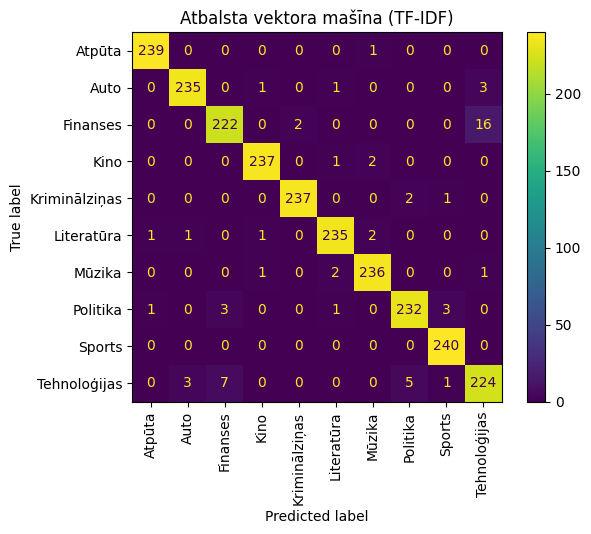
\includegraphics[width=0.75\textwidth]{AVM_TFIDF}
	\caption{Atbalsta vektora mašīnas pārpratuma matrica}
	\label{fig:AVM_TFIDF}
\end{figure}

\pagebreak
\section{Neironu tīklu implementācija}

Darba ietvaros tika izvērtētas un implementētas dažādas neironu tīklu arhitektūras. Tā kā tika nolemts pārbaudīt plašu spektru ar dažādiem apmācības algoritmiem – tika izvēlēts Python ietvars Keras, balstīts uz Tensorflow bāzes, kas palīdz ātri un sintaktiski vienkārši prototipēt dažādus modeļus. Neironu tīklu apmācība, vismaz sākotnēji, tika veikta uz autora datora, izmantojot viduvējas veiktspējas procesoru (AMD Ryzen 5700X) un 16GB RAM. Apmācība vienkāršākiem tīkliem šādi veicama diezgan efektīvi, tomēr sarežģītākas arhitektūras ar BiLSTM slāņiem vai BERT modeļa pielāgošana kļūst gan laikietilpīgāka (12+ stundu apmācība), gan ierobežota operatīvās atmiņas resursu dēļ. Šo iemeslu dēļ darba gaitā modeļu apmācība turpināta ar Google TPU v2, kas izstrādāts tieši neironu tīklu apmācībai un nodrošina krietni ātrakus apmācības laikus.

\subsection{Konvolūcijas neironu tīkli}
Konvolūcijas tīklu implementācijai tiek veidots Keras modelis ar secīgiem slāņiem – iegulšanas, viendimensiju konvolūcijas ar ReLU aktivizācijas funkciju, apvienošanas (globālā maksimuma), atmešanas, pilnīgi savienotais slānis gala klasifikācijas veikšanai. Ilustrēti ar papildus informāciju par izvēlētajām slāņu dimensijām varam apskatīt modeli \ref{fig:SingleLayerCNN} attēlā.

\begin{figure}[H]
	\centering
	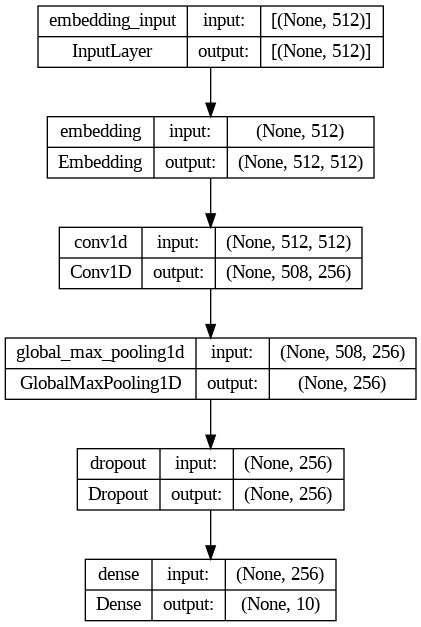
\includegraphics[width=0.4\textwidth]{SingleLayerCNN}
	\caption{Konvolūcijas neironu tīkla uzbūve}
	\label{fig:SingleLayerCNN}
\end{figure}

\pagebreak
Apmācību tiek veikta ar partijas izmēru kā 32, turpinot apmācību 10 epohos, saglabājot modeli posmos ar mazāko validācijas zuduma (validation loss) vērtību, mēģinot izvairīties no pārmērīgas pielāgošanas. Uz tekstiem pirms apmācības tiek veikta priekapstrāde - simbolu un stopvārdu atmešana. Akurātuma un zuduma evolūciju pa epohiem iespējams apskatīt \ref{fig:Accuracy_Loss_CNN_10epoch} attēlā.

\begin{table}[H]
\centering
\caption{\label{tab:score_cnn}}
\textbf{Veiktspējas mēri pielietojot konvolūcijas neironu tīklu\\}
\begin{tabular}{|l|l|}
\hline
Akurātums & F1 \\ \hline
0.9621 & 0.9620  \\ \hline
\end{tabular}
\end{table}

Pielietojot attēlā \ref{fig:SingleLayerCNN} ilustrēto konvolūcijas neironu tīkla uzbūvi tiek iegūti rezultāti kā \ref{tab:score_cnn} tabulā. Pārpratuma matricu iespējams apskatīt attēlā \ref{fig:CNN}, kur varam novērot līdzīgu kļūdu izplatību pa klasēm kā iepriekš apskatītos modeļos, arī ar šo pieeju visgrūtāk modelim ir atķirt tieši tehnoloģiju un finanšu ziņas.

\begin{figure}[H]
	\centering
	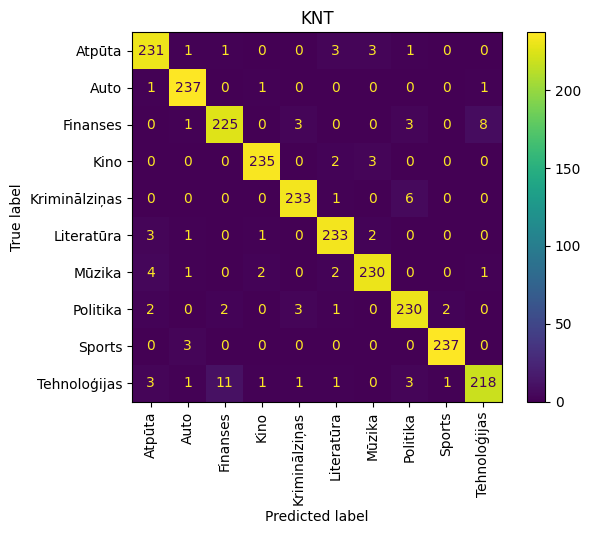
\includegraphics[width=0.75\textwidth]{CNN}
	\caption{Konvolūcijas neironu tīkli - pārpratuma matrica}
	\label{fig:CNN}
\end{figure}

\begin{figure}[H]
	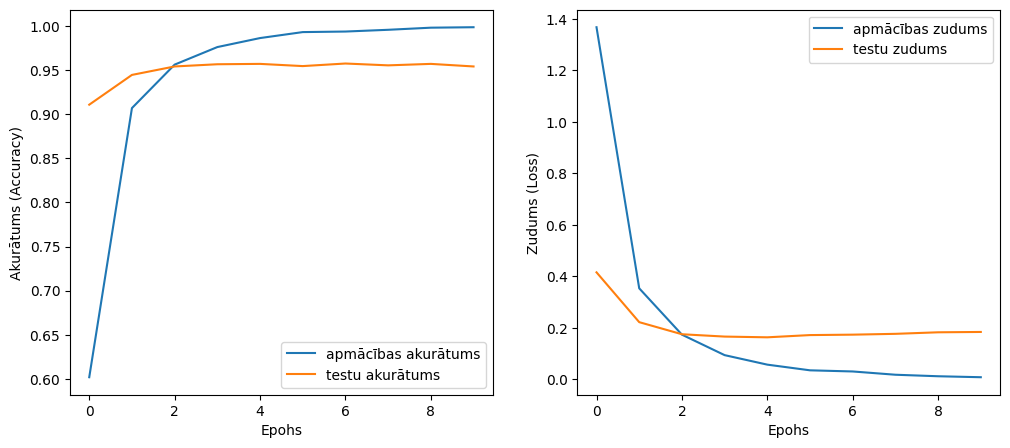
\includegraphics[width=\textwidth]{Accuracy_Loss_CNN_10epoch}
	\caption{Konvolūcijas neironu tīkli - novērtējums pa apmācības posmiem}
	\label{fig:Accuracy_Loss_CNN_10epoch}
\end{figure}

Mēģinot uzlabot modeļa veiktspēju tiek pielietota plaši citēta konvolūcijas neironu tīklu arhitektūra tekstu apstrādei no Kim Yoon \cite{kimYoonCNN}. Šīs arhitektūras galvenā ideja ir ieviest vairākus paralēlu konvolūcijas un apvienošanas slāņus ar dažādiem filtra izmēriem, vēlāk to rezultātus apkopojot. Galvenais iemesls – palīdzēt neironu tīklam apgūt dažādas iezīmes un likumsakarības tekstos, piemēram, mazāki filtri uztver vārdu kombinācijas, plašāki filtri – sarežģītākas valodas struktūras kā frāzes. Arī šāda pieeja tiek implementēta ar filtra izmēriem kā 4,5 un 6. Šī modeļa uzbūvi var apskatīt \ref{fig:MultiLayerCNN} attēlā.

\begin{figure}[H]
	\centering
	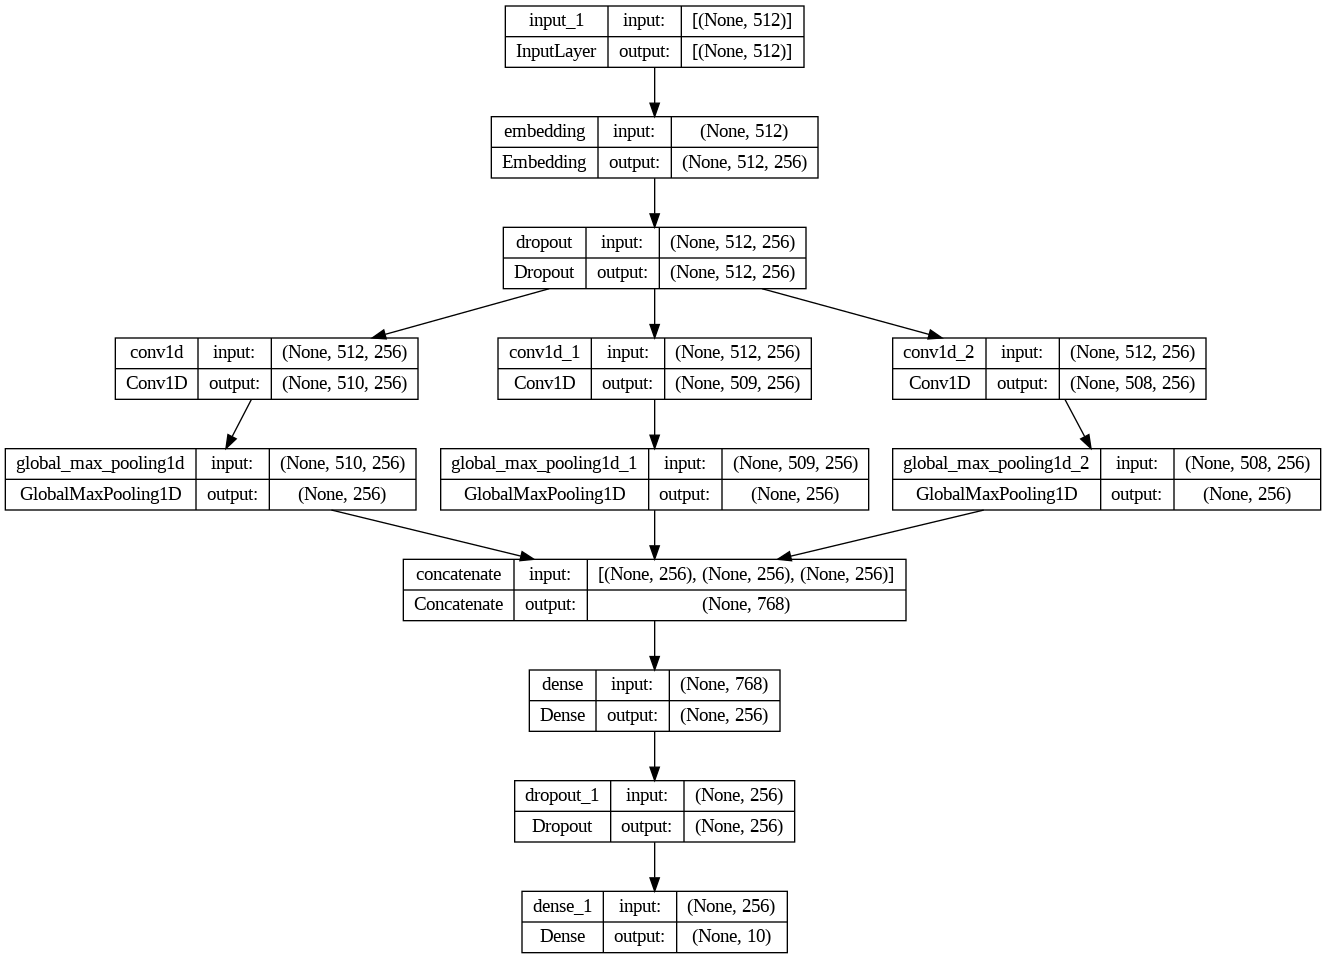
\includegraphics[width=0.85\textwidth]{MultiLayerCNN}
	\caption{Konvolūcijas neironu tīkla uzbūve - paralēla konvolūcija}
	\label{fig:MultiLayerCNN}
\end{figure}

\pagebreak
Modelis kurš apmācīts at augstākminēto arhitektūru nesiendza veiktspējas uzlabojumus, kā redzams \ref{tab:score_cnn_multi}tabulā.

\begin{table}[H]
\centering
\caption{\label{tab:score_cnn_multi}}
\textbf{Veiktspējas mēri -  konvolūcijas neironu tīkls ar parelēlu konvolūciju\\}
\begin{tabular}{|l|l|}
\hline
Akurātums & F1 \\ \hline
0.9517 & 0.9516  \\ \hline
\end{tabular}
\end{table}

\subsection{BERT}
Sākotnējais BERT modelis, kuru Google izstrādātāji jau bija apmācījuši un publicējuši, latviešu valodas ziņu apstrādei nav pielietojams, jo modelis apmācīts tikai uz angļu valodas tekstiem. Lai gan tikusi publicēta arī BERT uzbūves arhitektūra un modeli iespējams pašrocīgi apmācīt uz latviešu valodas tekstiem – šī darba ietvaros tas netiek veikts, jo šādai apmācībai nepieciešami ievērojami apmācības resursi ilgstošā laika posmā, kas autoram nav pieejami. Publiski gan palaik ir pieejams BERT modelis, kur apmācība uz latviešu valodas tekstiem jau ir veikta, to apmācījuši LU Matemātikas un informātikas institūta pētnieki Artūrs Znotiņš un Guntis Barzdiņš, modeli nosaucot par LVBERT. Tas ir apmācīts uz latviešu Wikipedia ierakstiem, tekstiem no valodas korpusa LVK2018, dažādiem ziņu rakstiem un to komentāriem, kas kopā veido 500 miljonu lielu tokenu kopu apmācībai \cite{lvbert}. Salīdzinot ar sākotnējo BERT modeli, LVBERT apmācības tokenu skaits ir vairāk nekā sešas reizes mazāks.

LVBERT, gluži kā citi BERT balstītie modeļi ir vispārināti un nav piemēroti tikai vienai problēmai – tos nepieciešams pielāgot konkrētai problēmai pirms to pielietošanas, šajā gadījumā - papildus tika pievienoti slāņi tieši klasifikācijas risināšanai. Papildus tekstu priekšapstrāde netika pielietota, jo tādējādi varam pazaudēt daļu no konteksta un saiknēm starp vārdiem, kas tieši ir viena no BERT modeļu spēcīgākajām pusēm.

Modeļa pielāgošana veikta 5 epohos ar apmācības ātrumu kā 2e-5 un partijas izmēru kā 32, šai kombinācijai pēc eksperimentiem ar dažādām parametru vērtībām uzrādot labākos rezultātus. Sākotnējā BERT publikācijā \cite{devlin2019bert} pielāgošana dažādiem GLUE uzdevumiem veikta ar partijas izmēru kā 32, 3 epohos un apmācības ātrumiem 5e-5, 4e-5, 3e-5 un 2e-5 (izvēloties labāko rezultējošo modeli katram uzdevumam).  Apskatot arī citas publikācijās \cite{sun2020finetune}, kur apskatīta BERT pielāgošana teksta klasifikācijai, apmācības ātrums kā 2e-5 uzrāda labākos rezultātus, kamēr lielāki ātrumi kā 4e-4 noved pie “katastrofālas aizmiršanas” problēmas, kur iepriekš apgūtā informācija tiek zaudēta veicot jaunu apmācību.

\begin{table}[H]
\centering
\caption{\label{tab:score_bert}}
\textbf{Veiktspējas mēri pielietojot BERT\\}
\begin{tabular}{|l|l|}
\hline
Akurātums & F1 \\ \hline
0.9704 & 0.9704  \\ \hline
\end{tabular}
\end{table}

Rezultātā iegūtā modeļa raksturojošie mēri skatāmi \ref{tab:score_bert} tabulā. Lai gan salīdzinot ar citiem neironu tīklu modeļiem tiek sasniegts rezultātu uzlabojums, tas nepārsniedz atbalsta vektora mašīnu akurātumu. Angļu valodas lielie valodu modeļi pārsvarā gūst krietni labākus rezultātus klasifikācijā, salīdzinot ar vienkāršākām metodēm. Daļējs izskaidrojums LVBERT veiktspējai varētu būt ievērojami mazākais tokenu skaits apmācības posmā, salīdzinot ar angļu valodas modeli.

\begin{figure}[H]
	\centering
	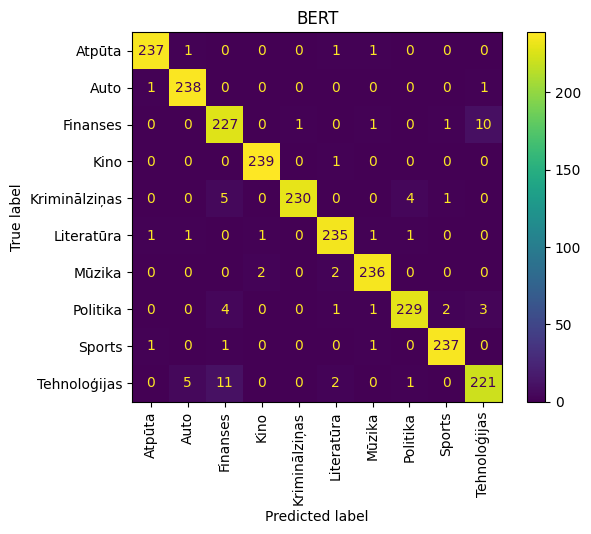
\includegraphics[width=0.75\textwidth]{Matrica_BERT}
	\caption{BERT - pārpratuma matrica}
	\label{fig:Matrica_BERT}
\end{figure}

Papildus apskatot pārpratuma matricu attēlā \ref{fig:Matrica_BERT}, BERT modelim var novērot līdzīgu klasifikācijas kļūdu sadalījums kā jau iepriekš apskatītajiem modeļiem.
